\documentclass[../main.tex]{subfiles}
\graphicspath{{\subfix{../figures/}}}

\begin{document}
\section{面向对象分析概述}
\textbf{学习目标}:
\begin{itemize}
  \item 掌握面向对象的基本思维方式、分析与设计的基本理论和方法;
  \item 掌握面向对象建模语言 UML
    及其设计软件、软件设计模式、面向对象程序设计语言;
  \item 采用面向对象方法设计实现小规模的应用程序. 课程内容包括:
    面向对象的基本概念,面向对象分析与设计的基本原则、方法与过程,面向对象设计模式.
\end{itemize}
\textbf{软件产品的主要类型}

从软件项目立项来源、用户群体等角度, 软件产品可划分为:
\begin{enumerate}
  \item 互联网软件:面向不特定人群,由互联网企业
    独立投资开发并免费开放给用户,通过服务、
    产品销售、广告等方式取得利润;搜索引擎、电商平台、即时通信、信息分发APP等.
  \item 通用软件:面向特定人群,由软件企业 独立投资开发并采用零售拷贝、许可证、
    使用时间等方式发售;ERP、办公套装软件、工具软件等.
  \item
    定制软件:由甲方(业主方)发起并提供开发经费,仅局限于某行业、某单位或部门等少数用户;XX集团运营管理系统、XX城市IOC平台.
\end{enumerate}
\textbf{软件开发一般过程}:提出问题→可行性 研究→需求分析→总体设计→详细设计→
编码与测试→试运行与培训→维护→ 评价.

\textbf{需求分析的主要活动}
\begin{enumerate}
  \item 与用户交流,获取拟开发系统的功能、性能、界面、
    安全等方面的要求;重点解决跨领域\textbf{沟通难}的问题。
    如某系统的需求:生成目标区内不同场点多概率水准的人造地震时程和天然地震时程.
  \item 梳理出\textbf{问题域}的业务流程、数据交换关系等信息;一般不涉及\textbf{计算机领域}的实现细节。针对上例中的需求:用什么数据、什么方法、怎么样的流程,生成什么样的结果
  \item 形成系统需求说明书(是软件开发所有后续工作的基础)。文字、图、表、动画、原型软件。
    针对上例中的分析:把分析结果表达出来
\end{enumerate}
数据交换与共享(横向,纵向),应用实现层,应用支撑层,数据资源层,基础设施层,支撑硬件基础设施.

\textbf{系统设计的主要活动}
\begin{enumerate}
  \item 总体设计:系统总体布局方案,软件系统总体结构的设计,数据存储的总体设计,计算机和网络系统方案的选择.
  \item 详细设计: 代码设计,数据库设计,人机界面设计,处理过程设计
  \item 系统实施进度与计划的制定
  \item 系统设计说明书的编写(是系统设计阶段的主要成果及下一阶段工作的基础).
\end{enumerate}
\subsection{传统的软件开发方法}
\textbf{功能分解法}:以功能为核心,对系统逐层进行分解,直至可直接实现的子功能,最后设计功能间的接口,和功能内部的数据结构、算法。
\begin{itemize}
  \item 优点:以功能为核心,较为直观、自然;逐层分解法与人类的思维模式相近,提高了开发效率。
  \item 缺点:功能和接口难以映射到问题领域中的事物;对需求变化的适应能力差。
\end{itemize}
\textbf{功能分解法示例, 成绩管理系统}:
\begin{enumerate}
  \item 教师信息管理:增删改查,导入教师信息;
  \item 课程管理: 管理课程基本信息,管理课程学生;
  \item 成绩维护:录入学生成绩,修改学生成绩.
\end{enumerate}
\textbf{信息建模方法}:以数据为中心的软件开发方法。
\begin{itemize}
  \item 优点:有关系数据库的良好数学基础,可保证系统的数据完整性、一致性;适合以数据处理为中心的软件系统;
  \item 缺点:对功能的刻画能力较弱;
\end{itemize}
\textbf{面向过程的结构化方法}:采用自顶向下,逐步求精的思想,把一个复杂问题的求解过程逐层、分阶段进行分解,使得每个阶段处理的问题都控制在人们容易理解和处理的范围内。
以模块为基础,以流程图、数据流图,数据字典,结构化语言,判定表,判定树等图形表达为主要建模手段。
\begin{itemize}
  \item 优点:开发过程的整体性和逻辑性较强;严格区分系统开发的阶段,分离逻辑设计和物理设计;每一阶段的工作成果是下一阶段的依据,便于系统开发的管理和控制;强调文档的规范化,可为系统的开发和维护提供良好支持
  \item 缺点:开发周期长,难以适应变化;分析与设计采用了不同的概念和表示法,相互转换困难.
\end{itemize}
\textbf{模块化}:系统划分为若干个模块,每个模块完成一个特定的功能,所有模块汇聚起来组成一个整体.
\begin{itemize}
  \item 模块:是一组能完成某个完整功能的程序语句,包括输入输出,逻辑处理功能,内部信息及其运行环境.
  \item 模块相对独立,模块间的接口简单
\end{itemize}
基于上述方法的软件开发过程存在两道\textbf{鸿沟}:
\begin{figure}[H]
  \begin{center}
    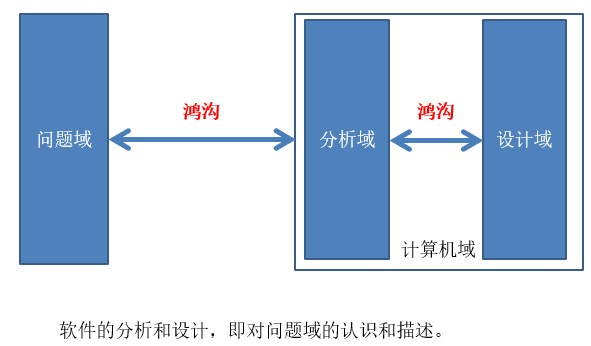
\includegraphics[width=0.50\textwidth]{1.jpg}
  \end{center}
\end{figure}
\subsection{面向对象技术概述}
\textbf{面向对象方法}是一种运用\textbf{对象、类、封装、继承、多态和消息}等概念来构造、测试、重构软件的方法。
\textbf{面向对象方法}是以\textbf{认识论}为基础,用\textbf{对象}来理解和分析\textbf{问题空间},并设计和开发出由对象构成的软件系统(\textbf{解空间})的方法。
\textbf{面向对象}是一种认识客观世界的思维方法.\textbf{面向对象}应用于软件开发,软件开发是将现实世界的问题映射为计算机领域的问题的过程.
面向对象技术的\textbf{核心}是\textbf{对象}。An object is anything that has a fixed shape or form, that you can touch or see, and that is not alive.
对象可代表现实世界的任何事物,概念。对象把数据结构和行为紧密结合在一起。\textbf{面向对象技术}是把一组对象有效地集成在一起形成软件的技术。

\textbf{OO的发展}
\begin{itemize}
  \item 最早20世纪50年代初,出现对象的概念.
  \item 1967年,产生第一个面向对象的语言Simula,提出了数据抽象和类的概念.
  \item 1972年,产生第二个面向对象的语言SmallTalk.
  \item 80年代,出现了Objective-C,Cpp,...
  \item 面向对象的分析,设计...
\end{itemize}
\textbf{面向对象的语言}包含4个基本的分支:
\begin{enumerate}
  \item 基于Smalltalk的; 包括smalltalk的5个版本,以Smalltalk-80为代表。
  \item 基于C的; 包括 objective-C, C++, Java
  \item 基于LISP的; 包括 Flavors, XLISP, LOOPS, CLOS
  \item 基于PASCAL的;包括 Object Pascal, Turbo Pascal, Eiffel, Ada 95
\end{enumerate}
\begin{itemize}
  \item 面向对象开发与面向过程开发对比,其主要好处不在于减少开发时间,而在于有利于问题域的分析,促进软件可重用,减少出错,利于软件维护。
  \item 面向对象的开发强调从问题域的概念到软件程序和界面的直接映射;心理学的研究也表明,把客观世界看成是许多对象更接近人类的自然思维方式。
  \item 对象比函数更为稳定;软件需求的变动往往是功能相关的变动,而其功能的执行者-对象通常不会有大的变动。
\end{itemize}
Example: $ y=kx+b $
\begin{itemize}
  \item int k; int b; float x;
  \item Formula(int k1, int b1, float x1)\{...\}
  \item float calculateY()\{return k*x+b;\}
\end{itemize}
Example: Tank
\begin{itemize}
  \item int x; int y; int width; int height; int speed; int direction;
  \item void move()(问题域); void fire(); void draw()(实现域).
\end{itemize}
用面向过程的结构化方法和面向对象方法来考察一个发票生成和打印系统.
\begin{itemize}
  \item 结构化方法:先分析发票生成和打印的过程,设计相应的数据结构,再设计基于该数据结构的函数;
  \item 面向对象方法:将发票看成一个对象,分析和设计对象的属性和方法;
\end{itemize}
\begin{figure}[H]
  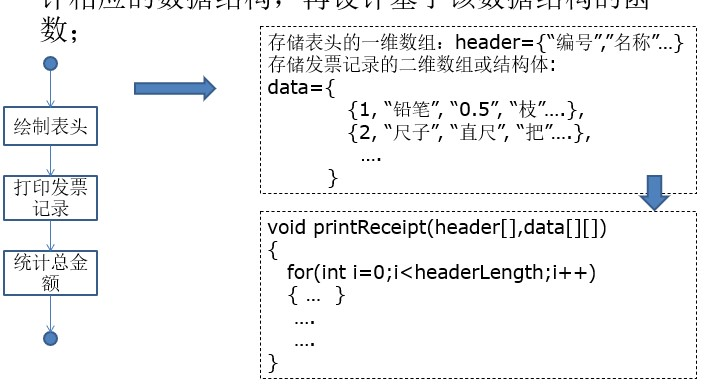
\includegraphics[width=0.50\textwidth]{2.jpg}
  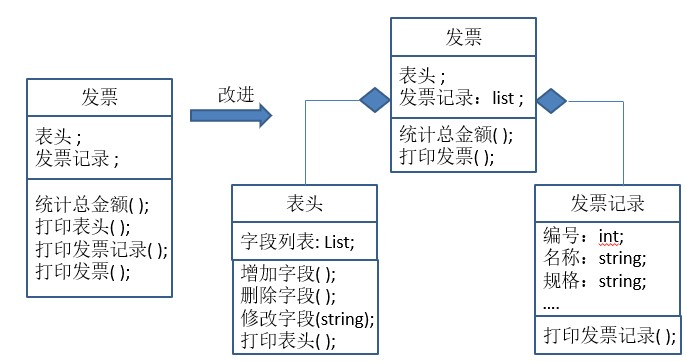
\includegraphics[width=0.50\textwidth]{3.jpg}
\end{figure}
\end{document}
